% \documentclass[journal]{IEEEtran}
\documentclass[journal,12pt,onecolumn,draftclsnofoot,]{sty/IEEEtran}
\usepackage{cite}
\usepackage[pdftex]{graphicx}
\usepackage{amsmath}
\usepackage{algorithmic}
\usepackage{array}
\usepackage{fixltx2e}
\usepackage{url}
% correct bad hyphenation here
\hyphenation{op-tical net-works semi-conduc-tor}


\begin{document}

\title{Neural Network-Based Speaker Identification \\ for Low-Power Devices}

\author{Skanda Koppula \\
        Supervisors: Dr. James Glass, Professor Anantha Chandrakasan}%

% The paper headers
\markboth{Masters of Engineering Thesis Proposal}%
{Speaker Identification for Low Power Devices}
% The only time the second header will appear is for the odd numbered pages
% after the title page when using the twoside option.

\maketitle

\section{Introduction}
Consumer devices using speech interfaces are growing in number and complexity. Small devices such as wearables, personal assistants, robots, and phones boast extensive voice-controlled interfaces that transact identity-specific data and are linked to personal profiles. Misuse of speech interfaces to maliciously execute illegitimate commands on such devices has been repeatedly demonstrated \cite{price_2016, feldman_2016}. In a particularly egregious example reported by popular press, a crafted TV commercial was able to activate voice-controlled personal assistants and deliver a voice command to execute an online purchase \cite{bbc_news_2017}. There is a strong motivation for speech interfaces linked to user profiles and private data to be simultaneously capable of speaker identification.

In the task of speaker identification (SID), a device learns the speech patterns unique to each of its owners, developing a model to distinguish between these identities and identities not in its set of owners (`the universe’). The device can subsequently use this model to perform forward inference, and identify whether an input voice command is from an authorized or a malicious party. Text-dependent SID refers to models trained to recognize persons speaking a specific keyword (e.g. `OK Google’). In contrast, text-independent models are able to distinguish a speaker for any spoken input.

Voice interfaces are common in small devices, where speech is an simple, intuitive avenue for user-device interaction. This presents a challenge: small devices are constrained in their power consumption, and relatedly, their memory capacity. Traditional SID algorithms consume on the upwards of hundreds of megabytes for model storage alone, well exceeding the limitations of many IoT devices.

This work focuses on developing an inference architecture for text-independent speaker identification that is applicable in scenarios constrained by power and latency, as is often the case in small devices. We will design new methods for speaker identification that achieve state-of-the-art accuracy but exhibit much smaller model sizes, to fit the constraints imposed by low-memory and low-power accelerators. We also aim to demonstrate the workability and comparative efficiency of this approach by implementation of our work in an FPGA.

In this proposal, we will first overview the background of speaker identification and neural network based speech inference (Section~\ref{prelim}). Second, we will detail the thesis's main objectives and salient subtasks (Section~\ref{problem}). Then we will then discuss related research and how this thesis builds on those prior works (Section~\ref{priorwork}). We conclude with a thesis timeline (Section~\ref{timeline}).


\section{Preliminaries}
\label{prelim}


\subsection{Front-End: Feature Extraction and VAD}
\label{frontend}
SID systems rely on pre-processing the raw waveform to capture salient information about the power spectrum of the utterance. Commonly used in SID are Mel-Frequency Cepstral Coefficients (MFCCs), features that capture the envelope of the frequency spectrum of an input waveform. To capture information emulating human perception of a waveform, MFCC extraction applies a Mel filterbank to the log-frequency spectrum; a Mel filter emulates filtering of frequencies based on frequency filtering performed by the human cochlea \cite{mfcc_pres}. Figure~\ref{mfcc} details the DSP pipeline for extracting MFCC features from an input waveform.


\begin{figure}
\centering
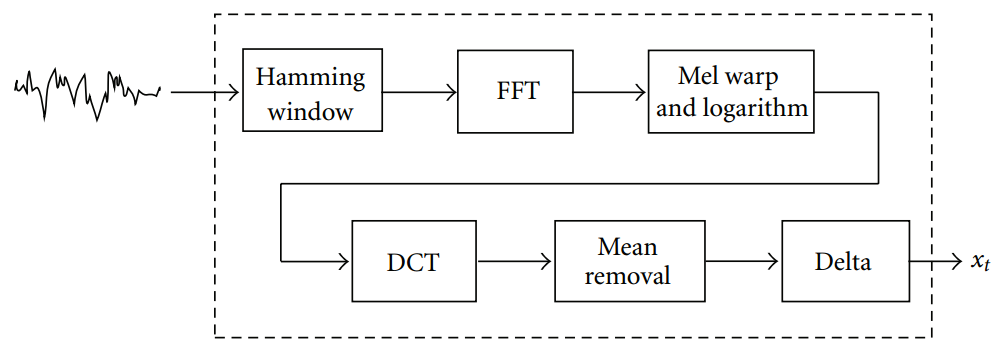
\includegraphics[width=0.9\textwidth]{figs/mfcc.png}
\caption{Example DSP pipeline for MFCC feature extraction. (1) Hamming windowing is first applied to avoid spectral leakage during the FFT (2) FFT is applied to capture frequency information (3) Mel filterbank is applied to the log-spectrum (4) Discrete Cosine Transform is used to extract real-number coefficients describing the envelope of the spectrum (5) The coefficients are mean-normalized (6) Optionally, the rate of change of coefficients (deltas) are appended to the coefficients to capture dynamic, contextual behavior of the time-varying signal. \cite{fpga_gmm}}
\label{mfcc}
\end{figure}

Non-voiced parts of the input signal provide no information for SID classification and serve to add noise and confuse backend classifiers. Nearly all text-independent SID systems apply voice-activity detection (VAD) to filter out segments of the waveform for which no human speech is detected. Pre-processing with VAD has been shown to produce marked improvements in automatic speaker recognition systems (ASR) and SID accuracy \cite{vad_hmf}. Additionally, in the context of ASR and SID hardware accelerators, integrating VAD allows designers to power-gate the speech classifier circuits, lowering the device’s total power draw. An example of this was demonstrated for ASR by Price et al. in 2016 \cite{price_dnn}.

There are three main kinds of VAD filters: energy-based, harmonicity-based, and modulation-frequency based. In low SNR conditions, triggering activation when the signal’s energy exceeds some threshold noise-floor is often sufficient to indicate the presence of speech. Two more robust methods of voice detection leverage the acoustic periodicity of human speech. Harmonicity-based (H) VAD measures the harmonics’ periodicity of the input signal. Modulation frequency (MF) based VAD measures the temporal rate of change of energy across different frequency bands. These measurements are fed into an upstream neural network classifier trained to detect voice activity with these inputs. A comparison of these approaches can be found in \cite{price_dnn}. We intend on re-using RTL source from \cite{price_wfst} and \cite{price_dnn} to implement a VAD that uses all three methods.

\subsection{Traditional Back-End: Gaussian Mixture Models and \textit{i-vectors}}
\label{tradbackend}
After feature vector extraction and VAD, SID systems rely on one of many algorithmic backends to drive classification of MFCCs. State-of-the-art systems frequently use of Gaussian Mixture Models (GMMs) due to its ability to mimic a wide variety of MFCC distributions. While we will not be using GMMs in this work, we briefly describe the method to familiarize an interested reader with the algorithmic benchmarks to which we will compare against. As we will discuss in Section~\ref{priorwork}, most attempts at low-resource SID have used GMM-based backends.

In a GMM-UBM system, the universe of all speakers is first modeled using a GMM (the universal background model, `UBM’). To learn the parameters of the UBM, expectation-maximization (EM) algorithm is used to fit the UBM to a public corpora of speech data covering thousands of speakers \cite{ubm2}. When the model wishes to learn a new `enrollee’ speaker, it shifts the UBM to better fit the enrollee’s input utterances using a few iterations of EM, forming a speaker-specific model. During evaluation, the system compares the likelihood of an input test utterance under the UBM versus under the speaker specific model \cite{ubm}.

State-of-the-art systems modify this simple evaluation procedure slightly. A `test-speaker’ GMM is trained using the input test utterance and a few iterations of EM. The distance between a speaker-specific model and the test-speaker model are compared using the concatenation of the Gaussian Mixture means (`supervectors’). Smaller cosine distances between supervectors indicates greater speaker similarity \cite{supervector}.

Unfortunately, storing, training, and comparing supervectors is computationally intensive and works poorly in practice: for a 2048-mixture GMM of 45 dimensions, the supervector dimensionality is extremely large: $45 \times 2048 = 92160$. Thus, a low-dimensionality intermediate representation of the supervector, the \textit{i-vector}, was formed to capture the difference between a UBM and a speaker-specific model in a low-dimensional subspace. For brevity, we leave a complete description of more optimized i-vector training, using sufficient statistics, to \cite{ivector_ss}. It is important to know, that transforming MFCCs to i-vector’s, and classifying i-vectors using PLDA is currently state of the art \cite{ivector_stateofart} \footnote{An alternative approach to train i-vectors is to use sufficient statistics of neural network posteriors instead of GMM statistics. This has been shown to result in modest accuracy gains. We leave the details to \cite{ivector_dnn_posterior}.}

Unfortunately, i-vector algorithms are not particularly amiable for low-resource SID evaluation. For example, with the standard i-vector size of 200, the i-vector extraction model requires 145 MB of storage \footnote{These models were trained using the popular speech toolkit Kaldi using publically available training scripts on the RSR and SRE corpora \cite{kaldi, sre, rsr}}. Even reducing the precision from 32-bit float to 8-bit (at an 8% cost in recognition accuracy), the model size drops to 36 MB, too large to fit in an accelerator’s SRAM.

\subsection{Contemporary Back-End: Neural Networks}
\label{backend}
Neural networks demonstrate promise as an alternative back-end MFCC classifier. In addition to achieving state-of-the-art in image recognition, language translation, and drug discovery \cite{imagenet, translation, drugs}, end-to-end neural networks have demonstrated record-breaking performance in a number of speech related tasks: speech recognition, language recognition, and text-dependent speaker identification \cite{speechrec, lidsid, smallfootprint}. In this work, we intend to use recurrent and feedforward neural network architectures as our SID backend model.

Particularly attractive about a deep neural networks (DNNs) is the powerful ability to compress model size while experiencing little to no loss in accuracy. Through a combination of pruning, quantization, and parameter encoding, compression ratios of up 510x have been demonstrated and implemented in FPGA for image recognition networks \cite{squeezenet}. In speech recognition, 20x reduction in sizes have been achieved (from 51 MB to 3.7 MB) using weight-matrix factorization \cite{smallfootprintasr}. In both these cases, no loss of accuracy was experienced. Additionally, architecture level optimizations (redesigning the network structure) provide another avenue for model compression; we demonstrate that this affords an addition 10x reduction in our speaker identification network size. Unlike i-vector models, which have resisted attempts to reduce their memory bandwidth and computational overhead, neural networks show promise as a candidate for a model that would fit in SRAM \cite{deepcompression}.

\section{Problem Statement and Tasks}
\label{problem}
The goal of this work is to develop an digital inference architecture for text-independent speaker identification that is applicable in scenarios constrained by power, memory, and latency. We plan to demonstrate our algorithms and architecture in FPGA. By using various model optimizations, we aim to achieve a system that is comparable to or exceeds i-vector SID systems in recognition accuracy.

The core of this work is two-fold. First, we will design and train a low-depth, small footprint SID network that can be efficiently evaluated on resource-constrained devices (such as a low-power accelerator). Secondly, we will be developing generalizable hardware designs to perform inference on the network we develop.

\begin{figure}
\centering
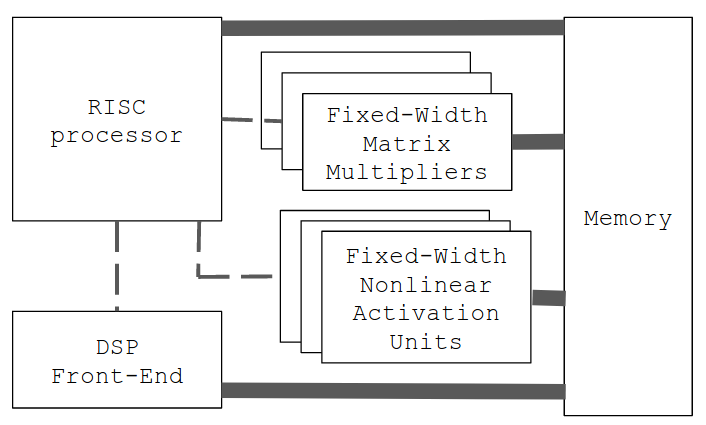
\includegraphics[width=0.9\textwidth]{figs/architecture.png}
\caption{Inference architecture for re-programmable networks for SID. Thick edges between components represent data lines, dashed lines represent control signal lines.}
\label{architecture}
\end{figure}

In the process, there are a number of subtasks that the project will need to hit:
\begin{enumerate}
\item As noted by \cite{price_dnn} and \cite{deepcompression}, one challenge of low-power network inference is keeping the network size small enough to fit in SRAM; of primary focus is model size, for which we will need to design and benchmark a competitive SID network less than 8 MB. For this we will experiment with new network architecture designs (e.g. using long short-term memory networks), edge pruning \cite{deepcompression}, and weight quantization \cite{quantize}. One particularly promising network architecture design we found during experimentation is the use of attention to direct a small recurrent network to focus on the most informative parts of an input signal \cite{attention} (Figure~\ref{attentionnet}).

\item We will study the effects of forcing fixed-point, integer arithmetic on the recognition accuracy of our SID network. The signed floating-point parameters typically used in networks complicates digital logic, so we seek to operate in a fixed-point, integer world. In small experiments, our rounded model experienced drops in recognition rates from 3-5\%, requiring us to retrain the network in the fixed-point parameter domain. To compensate for accuracy losses, we will also experiment in applying Dense-Sparse-Dense training methods \cite{dsd}.

\item Our goal is for our digital architecture to be generalizable; if we decide to change the SID network architecture post-synthesis and placement, we should be able to do so. This would involve writing a small compiler to translate network architectures to RISC instructions that execute on a RISC processor that orchestrates the correct sequence of commands to other components in the design (e.g. matrix multipliers, non-linear activation units, etc.). Figure~\ref{architecture} illustrates the target digital architecture. As is currently implemented, the network architecture is hard-coded in RTL.

\item Some effort has been made to integrate phonetic information into the SID i-vector systems. Such work attempts to normalize out intra-speaker phonetic variation, and solely capture inter-speaker variation \cite{lidsid, multitaskasr}. Additions such as bottleneck features and DNN-based sufficient statistics have been proposed to the basic i-vector system allowing for modest gains in accuracy. We have considered applying the same phoneme-integration techniques to our network model; the cost of this would be increased model size. We intend to run small benchmarks to understand the model complexity-performance ratio of such an addition.

\item Last but not least, we will need to demonstrate designs for front-end processing components (for which there is prior work \cite{price_dnn, price_wfst, mfccchip}), and integrate this component into our network evaluation designs.

\end{enumerate}

\begin{figure}
\centering
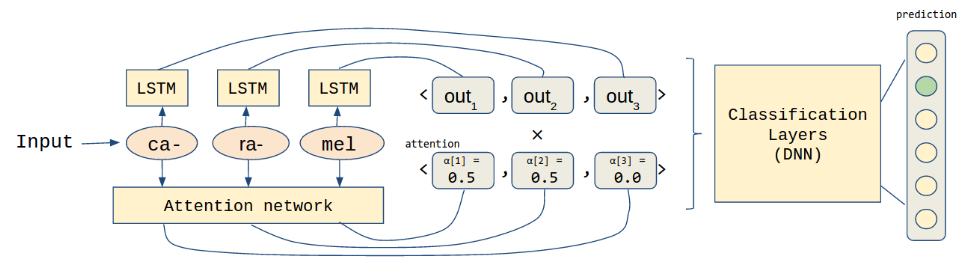
\includegraphics[width=0.9\textwidth]{figs/attentionnet.png}
\caption{Network architecture with small recurrent LSTM module and an attention mechanism. Based on various SID benchmarks, we’ve found this topology to have a promising model complexity-accuracy ratio.}
\label{attentionnet}
\end{figure}

\section{Prior Work}
\label{priorwork}

\subsection{Neural Network Based SID}
Several groups have studied the application of end-to-end neural networks for SID. For text-dependent SID, \cite{smallfootprint} and \cite{svattn} have demonstrated network architectures that exceed the accuracy of i-vector systems. These networks, however, exceed 70 MB in size, and not suitable for direct adaptation \footnote{Interestingly,  both these models have been deployed to consumer electronics, in the Google Home personal assistant and Windows phones, respectively. The devices do not do inference locally; rather, they communicate with cloud services that perform forward evaluation through the network for them.}

Prior art on neural-network based text-independent SID is a bit more sparse. \cite{tisv} describes a Siamese network for text-independent speaker verification (the one-vs-universe case of speaker identification). The authors report mixed accuracy benchmarks as compared to i-vector systems on a proprietary dataset. In this work, we aim to achieve across the board accuracy gains against the i-vector system on standard open SID datasets.

\subsection{SID on Resource-Constrained Devices}
\cite{sidfpga} implements a very basic SID system in FPGA. The core recognition algorithm uses the the cosine distance between downsampled MFCC feature vectors. Accuracy of the system was not benchmarked. \cite{svmfpga} replaces the cosine distance classifier with an SVM, again reporting no accuracy benchmarks. Both works implement their own DSP front-end as the crux of the papers.

More recently, \cite{fpga_gmm} implements a complete GMM/UBM text-independent SID system on FPGA. They suffer a 5\% accuracy reduction because of losses due to fixed-point integer approximations in the GMM mean and covariance matrices.

To the best of our knowledge, besides general purpose network evaluators such as EIE and Eyeriss, there has been no previous work that use perform neural-network based SID on resource-constrained devices \cite{eie, eyeriss}. Both EIE and Eyeriss are much larger in area than what is required for SID, and lack a SID front-end.

\section{Timeline}
\label{timeline}

Previous and ongoing work:
\begin{enumerate}
\item Collect and pre-process YOHO, SRE, and RSR datasets. Become familiar with Kaldi (September 2016, Done)
\item Train GMM/UBM and i-vector models on SRE and RSR for comparison purposes (October 2016, Done)
\item Implement PLDA and neural network backend with i-vector model. Survey literature on end-to-end DNN approaches to SID and gauge feasibility. Research the costs and benefits of building i-vector vs. neural network SID for low-power. (November 2016, Done)
\item Implement first feedforward network. Test on YOHO datasets. Debug the extremely poor accuracies. Explore using AWS GPU machines for training (December 2016, Done)
\item Demonstrate a working SID demo on an ARM embedded device using neural network/i-vector fusion backend. Get setup on SLS GPU machines.  (January 2017, Done)
\item Create network compression scripts that translate weights to 8-bit integers by using a quantization encoding scheme (February 2017, Done)
\item Continue attempts to make model smaller. Implement LSTM/recurrent networks as alternative to less-accurate feedforward networks. Debug poor accuracies. Review Bluespec, obtain Xilinx SoC. (March 2017, Done)
\item Various fixes to LSTM network. Implement attention mechanism on hunch. Make designs for matrix multiplier, ReLU in BSV (April 2017, Done)
\item Convert BSV to Vivado HLS in order load modules as IP into Vivado to program Xilinx SoC. Wire multipliers and activations together to obtain simple neural network architecture in hardware, on the Xilinx FPGA. (Early May 2017, Done)
\item Read manuals to figure out how to feed in audio data over UART from computer to the ARM chip on the Xilinx SoC, and then subsequently to the FPGA. Continue expanding simple network in Vivado, write test bench. Convert previously trained network weights to 8-bit integer using my scripts and benchmark. (May 2017, Ongoing)
\end{enumerate}

Future work:
\begin{enumerate}
\item Demonstrate SID on Xilinx SoC, using previous week’s work (hardcoded network topology, front-end on computer) (early June 2017, Ongoing)
\item Benchmark small footprint attention network SID on more datasets, comparison i-vector vs. attention network, write-up for ICASSP publication.  (June 2017, Ongoing)
\item Read and familiarize self with Michael’s front-end DSP RTL source (VAD and feature extraction). Plan out how to integrate (July 2017)
\item Obtain documentation about RISC processor design from Chiraag. Familiarize self with how to execute programs on processor. Think about procedure for converting a Tensorflow network topology into program on RISC processor. (August 2017)
\item Implement and test front-end DSP RTL on Xilinx SoC (September 2017)
\item Implement and test general purpose matrix multiplier modules and activation modules (Figure~\ref{architecture}), based on previous Vivado HLS work. Prepare for ICASSP submission. (October 2017)
\item Implement and test neural network to RISC instructions compiler (November 2017)
\item Piece together module, debug and test, and demo adjustable neural network based SID on Xilinx FPGA (December 2017)
\item Work with Chiraag on hardware accelerated encrypted-DNN evaluation (January 2018)
\item Port designs from encrypted DNN to SID designs to protect input and the speaker model (February, March 2018)
\item Explore other applications of the FPGA designs: running language ID and/or KWS on the same chip, using the same front-end, but loading different model (April, May 2018)
\end{enumerate}

\newpage

\bibliographystyle{sty/IEEEtran}
\bibliography{IEEEabrv,citations}

\end{document}


